%& --include-directory=/tex

\documentclass[a4paper,danish]{article}

\usepackage[utf8]{inputenc} % Skal passe til editorens indstillinger
\usepackage[danish]{babel} % danske overskrifter
\usepackage[]{biblatex}
\bibliography{bibbase}
\usepackage[T1]{fontenc} % fonte (output)
\usepackage{lmodern} % vektor fonte
\usepackage{graphicx} % indsættelse af billeder
\usepackage{epstopdf} %Tilfj "--enable-write18" i argumentet for LaTex build. Dette vil konvertere .eps figurer til pdf-format
\graphicspath{{./picture/}} % stivej til bibliotek med figurer
\usepackage{subfigure} %Til gruppering af figurer
\usepackage{mathtools} % matematik - understøtter muligheden for at bruge \eqref{}
\usepackage{hhline} % 
\usepackage{url} %Url's der ser korrekt ud og tillader brug af tilde
\usepackage{multirow} %Lader en tabelcelle fylde flere rækker
\usepackage[toc,page]{appendix} %Sørger for at bruge bogstaver til appendix istedet for talrækkefølgenn
\textwidth = 400pt
\marginparwidth = 86pt
\hoffset = -25pt
\voffset= -10pt
\textheight = 630pt
\newcommand{\HRule}{\rule{\linewidth}{0.5mm}}
\usepackage{fancyhdr}
\usepackage[plainpages=false,pdfpagelabels,pageanchor=false]{hyperref} % aktive links
\hypersetup{%
  pdfauthor={Insert author},
  pdftitle={Insert title of assignment},
  pdfsubject={Insert subject of assignment}}
\usepackage{memhfixc}% rettelser til hyperref

%%%%grafer
\usepackage{tikz}
\usepackage{pgfplots}
%\pgfplotsset{compat=1.4}



\fancyhf{} % tom header/footer
\fancyhfoffset{20pt}
\fancyhfoffset{20pt}
\fancyhead[OL]{Hyttebums 2012 ansøgning \\ Simon Dam Grønnegaard \& Morten Halvorsen}
%\fancyhead[OC]{Date \\ insert date}
\fancyhead[OR]{Danmarks Tekniske Universitet\\ DTU Hyttebums}
\fancyfoot[FL]{}
\fancyfoot[FC]{\thepage}
\fancyfoot[FR]{}
\renewcommand{\headrulewidth}{0.4pt}
\renewcommand{\footrulewidth}{0.4pt}
\pagestyle{fancy}

% How to make ref to books or urls in bib
%\citetitle[fx: page 1]{name of ref in bib}

\begin{document}
\begin{titlepage}
\centering \parindent=0pt
%\newcommand{\HRule}{\rule{\textwidth}{1mm}}
\vspace*{\stretch{1}} \HRule\\[1cm]\Huge
Hyttebums 2012 ansøgning\\[0.7cm]
\LARGE Holy \& Moly - videnskabelig undersøgelse af hyttebumskandidater\\[1cm]
\HRule\\[2cm]  
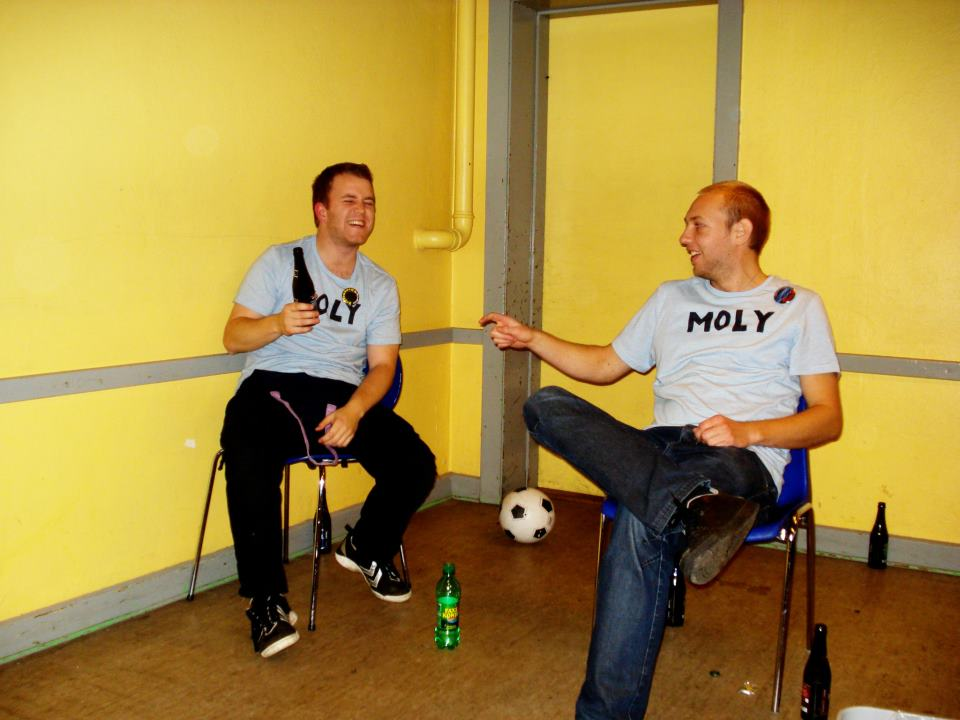
\includegraphics[width=8cm]{HolyMolyBowling}\\ %Use this if you want a picture on the frontpage

\Large Simon Dam Grønnegaard aka Holy\\ 
Morten Halvorsen aka Moly


\vspace*{\stretch{1}} \normalsize %
\begin{flushleft} \Large
DTU Housebums\\
Department of housebums\\
\today \end{flushleft}
\vspace*{\stretch{2}} \normalsize
\begin{flushright}
\includegraphics[width=2cm]{./pf}\\
\end{flushright}
\end{titlepage}
\newpage
\tableofcontents
\newpage

\section{Introduktion}
Denne rapport beskriver og diskuterer \HM som mulige Housebums 2012. Først afklares kort teorien omkring kødvalg, som enhver Housebum bør have viden omkring. Herefter gennemgås de praktiske erfaringer og evner de to ansøgere besidder med særlig vægt på alt inden for madlavningsdisciplinen. Til sidst opsummeres og besvares de påkrævede dele af ansøgningen i konklusionen. 

Alt er dokumenteret og underbygget med referencer til pålidelige kilder.

\include{teory}

\section{Erfaring}
En samlet liste af erfaringen de to kandidater har indenfor feltet hyttebombing indenfor Polyteknisk Forening:

\subsection{Studiestarten}
\begin{enumerate}
\item Vektor 2006
\item CSK 2007
\item CSK 2008
\item Vektor 2008
\item CSK 2009
\item Vektor 2009
\end{enumerate}

\subsection{Madhold}
\begin{enumerate}
\item vOPtur 2008
\item Rustur 2009
\item hyttetur ELKO nystartende 2010
\item S-husets hyttetur 2011
\item OPtur 2011
\item Rustur 2011
\item hyttetur ELKO nystartende 2011
\item S-husets hyttetur 2012
\end{enumerate}


\subsection{Arrangør af ture}

\begin{enumerate}
\item Rustur 2006
\item HerreHyggeHyttetur ELKO 2007 
\item OPtur 2007
\item Rustur 2007
\item HerreHyggeHyttetur ELKO 2008
\item OPtur 2008
\item Rustur 2008
\item hyttetur ELKO nystartende 2008
\item HerreHyggeHyttetur ELKO 2009
\item OPtur 2009
\item Rustur 2009
\item hyttetur ELKO nystartende 2009
\item HerreHyggeHyttetur ELKO 2011
\item HerreHyggeHyttetur ELKO 2012
\end{enumerate}

\subsection{PF kompetancer}
\begin{enumerate}
\item Formand for ELKO rådet 2007-2009
\item UddanelsesPolitisk Råd 2007-2012
\item ISN Fotonik 2007-2012
\item Hegnet 2007->
\item Hegnet Formand 2007-2008
\item Fællesrådet 2009+2011-2012
\item Fællesrådets ForretningsUdvalg 2009-2012
\item PF's Bestyrelse 2010
\item Formand for ELKO rådet 2011-2012
\item Akademisk Råd (DTU) 2011-2012
\end{enumerate}



\section{Konklusion}
Det kan konkluderes at Holy \& Moly \texttrademark er yderst velegnet til at besidde titlen Housebums. Specielt skal der lægges vægt på følgende observationer i forhold til ansøgninger til Housebums:
\begin{itemize}
\item Begge besidder kørekort til minimum 2057
\item Alderen på los Housebums er hhv. $824 \cdot 10^6 s$ (Holy) og $789 \cdot 10^6 s$ (Moly) (26år + 25år) \footnote{Opgivet i forhold til Housetrips starttidspunkt}
\item Telecommunication, næstsidste semester (Holy).\\
Elektroteknologi med speciale i akustik, det løber det op (10. semester) (Moly) 
\item Fleksibiliteten med hensyn til hytte er enorm gående eksponentielt mod $\infty$
\item Holy \& Moly \texttrademark er et brand og kan derfor ikke splittes op uden stort tab af madglæde blandt de spisende. Ligesom at tage Gøg uden Gogge, Spøg uden Skæmt, Jack Black uden Kyle Gass, Monty uden Python og Casper uden Mandrilen; det funger \footnote{For rigtig udtalelse: \url{http://www.youtube.com/watch?v=yVRWQ86DSjo}} bare ikke. 
\end{itemize}

%End of the document, inserting bib and appendix
\newpage
\nocite{*}
\printbibliography

\newpage
\appendix

\end{document}
